\immediate\write18{makeindex main.nlo -s nomencl.ist -o main.nls}
\documentclass[12pt,a4paper]{report}
\usepackage[utf8]{inputenc}
\usepackage{vietnam}
\usepackage[left=3cm, right=2.2cm, top=2.5cm, bottom=2.5cm]{geometry}
\usepackage{amsmath}
\usepackage{float}
\usepackage{amssymb} 
\usepackage{graphicx} 
\usepackage[hidelinks, unicode]{hyperref}
\usepackage[labelsep=period]{caption}
\usepackage[table]{xcolor}
\usepackage{titletoc}
\usepackage{etoc}
\usepackage{mathptmx}
\usepackage{sectsty}
\usepackage{multirow}
\usepackage{booktabs, tabularx}
\usepackage{courier}
\usepackage{subfig}
\usepackage{nomencl}
\usepackage{titlesec}
\usepackage{enumitem}
\usepackage{anyfontsize}
\usepackage[fontsize=13pt]{scrextend}
\newcommand{\code}[1]{\texttt{#1}}
\renewcommand{\baselinestretch}{1.5}
\renewcommand{\nomname}{Danh mục ký hiệu và viết tắt}


\makenomenclature
\makeatletter
\titlecontents{chapter}[3cm] % <-- seems to set some specific left margin
{\color{black}\bfseries\addvspace{3mm}}
{\makebox[0cm][r]{\MakeUppercase\@chapapp\hspace{.5em}\thecontentslabel\hspace{0.75cm}}}
{} %     ^^^ pretendously zero width box puts its contents in the left margin
{\hfill\makebox[-2cm]{\thecontentspage}}  % 3cm = twice 1.5cm
\chapternumberfont{\Large}
\chaptertitlefont{\Large}

\titleformat{\chapter}[hang] 
{\normalfont\fontsize{14}{15}\bfseries}{CHƯƠNG \thechapter.}{1em}{} 
\titlespacing*{\chapter}{0pt}{-7pt}{7pt}

\titleformat{\section}
{\normalfont\fontsize{13}{15}\bfseries}{\thesection.}{1em}{}
\titlespacing*{\section}{0pt}{-5pt}{-6pt}  

\titleformat{\subsection}
{\normalfont\fontsize{13}{15}\bfseries\itshape}{\thesubsection.}{1em}{}
\titlespacing*{\subsection}{0pt}{-20pt}{-6pt}

\titleformat{\subsubsection}
{\normalfont\fontsize{13}{15}\itshape}{\thesubsubsection.}{1em}{}
\titlespacing*{\subsubsection}{0pt}{-20pt}{-6pt}


\newcommand{\subsubsubsection}[1]{\paragraph{#1}\mbox{}\\}


\setlist[itemize]{itemsep=-0.3em, topsep=0pt}
\setlength\parindent{0pt}
\setlength{\parskip}{10pt}
\setcounter{secnumdepth}{4}
\setcounter{tocdepth}{4}
\geometry{letterpaper}

\begin{document}
\chapter{TỐI ƯU HÓA KHAI THÁC CHO GIẾNG X}

\section{Giới thiệu phần mềm PIPESIM}
PIPESIM là phần mềm mô phỏng do Schlumberger phát triển, có chức năng thiết kế và phân tích hệ thống khai thác của các giếng dầu và giếng khí. Hình \ref{fig:production_system} thể hiện mô hình dòng chảy đa pha từ trong vỉa qua các thành phần của hệ thống khai thác tới các thiết bị bề mặt cho phép phân tích hệ thống khai thác một cách toàn diện.
	\begin{figure}[h]
		\centering
		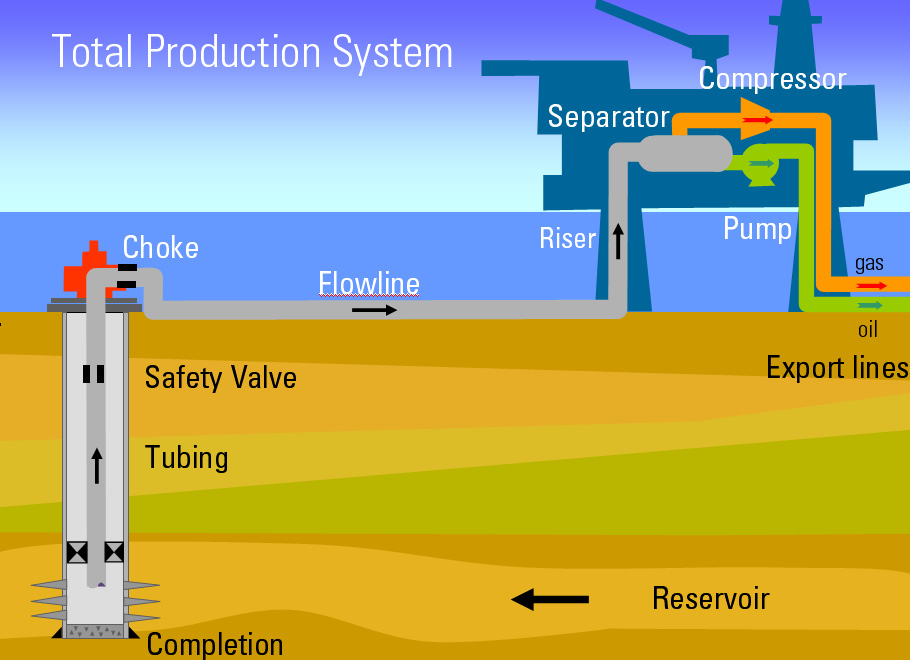
\includegraphics[scale=0.6]{Fig/production_system.png}
		\caption{Toàn bộ hệ thống cơ bản của một giếng khai thác}
		\label{fig:production_system}
	\end{figure}
\newline
PIPESIM thường được sử dụng cho phân tích vỉa, khai thác hay các thiết bị kĩ thuật. Một số chức năng chính của PIPESIM như sau:
	\begin{itemize}
		\item Phân tích các mô hình đặc tính giếng
		\item Phân tích điểm nút
		\item Thiết kế hệ thống khai thác dầu bằng khí nén
		\item Xây dựng hệ thống ống dẫn và thiết bị
		\item Phân tích đưa ra kế hoạch phát triển mỏ
		\item Tối ưu hóa khai thác.
	\end{itemize}
Phiên bản được nhóm tác giả sử dụng là PIPESIM 2017.1 có nhiều sự thay đổi về giao diện người dùng tuy nhiên các tính năng chính không có sự thay đổi nhiều so với các phiên bản cũ hơn.

\section{Mô hình khai thác của giếng X trên Pipesim}
\subsection{Dữ liệu đầu vào của giếng X}

Các thông số đầu vào của mô hình bao gồm thông số vỉa, lưu chất vỉa (Black-Oil), tubing, khoan định hướng, ống chống, các thiết bị bề mặt, các thiết bị lòng giếng, khai thác nhân tạo, hoàn thiện giếng và thông số truyền nhiệt được thể hiện qua các Bảng \ref{tab:reservoir_data} đến Bảng \ref{tab:surface_equipment}.

\begin{table}[h]
\caption{Thông số vỉa}\label{tab:reservoir_data}
\begin{tabularx}{\textwidth}{@{}XXX@{}}
\toprule
Thông số            & Dữ liệu & Đơn vị        \\ \midrule
Áp suất vỉa    & 3600 & psia        \\
Nhiệt độ vỉa & 200  & degF        \\
Chỉ số khai thác      & 9.4  & STB/(d.psi) \\ \bottomrule
\end{tabularx}
\end{table}

\begin{table}[h]
\caption{Tính chất lưu chất vỉa}\label{tab:fluid_properties}
\begin{tabularx}{\textwidth}{@{}XXX@{}}
\toprule
Thông số & Dữ liệu & Đơn vị    \\ \midrule
Watercut   & 10   & \%      \\
GOR        & 500  & SCF/STB \\
Tỉ trọng khí    & 0.8  & S.G     \\
Tỉ trọng nước  & 1.05 & S.G     \\
API        & 36   & dAPI    \\ \bottomrule
\end{tabularx}
\end{table}
\nomenclature{GOR}{Tỉ số khí dầu}

\begin{table}[h]
\caption{Các thông số của tubing}\label{tab:tubing_params}
\begin{tabularx}{\textwidth}{@{}XXX@{}}
\toprule
Thông số         & Dữ liệu & Đơn vị \\ \midrule
Độ sâu đo        & 8600    & ft     \\
Đường kính ngoài & 4.5     & in     \\
Đường kính trong & 3.476   & in     \\
Độ dày thành ống & 0.271   & in     \\
Độ nhám          & 0.001   & in     \\ \bottomrule
\end{tabularx}
\end{table}

\begin{table}[h]
\caption{Các thông số khoan định hướng}\label{tab:wellbore_data}
\begin{tabularx}{\textwidth}{@{}XX@{}}
\toprule
Độ sâu đo đạt (ft) & Độ sâu thực (ft) \\ \midrule
0       & 0        \\
1000    & 1000     \\
2500    & 2450     \\
5000    & 4850     \\
7500    & 7200     \\
9000    & 8550     \\ \bottomrule
\end{tabularx}
\end{table}

\begin{table}[h]
\caption{Các thông số truyền nhiệt}\label{tab:heat_transfer}
\begin{tabularx}{\textwidth}{@{}XX@{}}
\toprule
Độ sâu thực (ft) & Nhiệt độ môi trường (degF) \\ \midrule
0                & 50                         \\
8550             & 200                        \\ \bottomrule
\end{tabularx}
\end{table}

\begin{table}[h]
\caption{Thiết bị khai thác nhân tạo}\label{tab:gaslift_valve}
\begin{tabularx}{\textwidth}{@{}XXXX@{}}
\toprule
Tên        & Độ sâu đo (ft) & Lưu lượng bơm ép & Đơn vị  \\ \midrule
Bơm ép khí & 8000           & 0.1              & mmscf/d \\ \bottomrule
\end{tabularx}
\end{table}

\begin{table}[h]
\caption{Các thông số của ống chống}\label{tab:casing_data}
\begin{tabularx}{\textwidth}{@{}XXX@{}}
\toprule
Thông số         & Dữ liệu & Đơn vị \\ \midrule
Độ sâu đo        & 9000    & ft     \\
Đường kính ngoài & 8.625   & in     \\
Đường kính trong & 7.511   & in     \\
Độ dày thành ống & 0.557   & in     \\
Độ nhám          & 0.001   & in     \\ \bottomrule
\end{tabularx}
\end{table}

\begin{table}[h]
\caption{Các thiết bị lòng giếng}\label{tab:downhole_equipment}
\begin{tabularx}{\textwidth}{@{}XXXX@{}}
\toprule
Thiết bị      & Tên              & Trạng thái & Độ sâu đo (ft) \\ \midrule
Packer        & Packer 1         & Hoạt động  & 8500           \\
Packer        & Packer 2         & Hoạt động  & 7000           \\
Choke         & Choke 1          & Hoạt động  & 7500           \\
Ống bao trượt & Sliding Sleeve 1 & Hoạt động  & 8000           \\ \bottomrule
\end{tabularx}
\end{table}

\clearpage

\begin{table}[h]
\caption{Các thông số hoàn thiện giếng}\label{tab:well_completion}
\begin{tabularx}{\textwidth}{@{}XXXX@{}}
\toprule
Tên          & Độ sâu đo (ft) & Loại hoàn thiện & Trạng thái \\ \midrule
Completion   & 8800           & Bắn mở vỉa      & Hoạt động  \\
Completion-1 & 8000           & Bắn mở vỉa      & Không hoạt động  \\ \bottomrule
\end{tabularx}
\end{table}

\begin{table}[h]
\caption{Thông số thiết bị bề mặt}\label{tab:surface_equipment}
\begin{tabularx}{\textwidth}{@{}XXXX@{}}
\toprule
                         & Thông số         & Dữ liệu & Đơn vị \\ \midrule
\multirow{6}{*}{Ống dẫn} & Đường kính ngoài & 3.5     & in     \\
                         & Đường kính trong & 2.9     & in     \\
                         & Độ dày thành ống & 0.3     & in     \\
                         & Độ nhám          & 0.0018  & in     \\
                         & Tỉ lệ uốn        & 0       &        \\
                         & Length           & 1000    & ft     \\
Choke                    & Độ mở van        & 1       & in     \\ \bottomrule
\end{tabularx}
\end{table}

\vspace{15pt}
\subsection{Mô hình khai thác của giếng X}

Mô hình khai thác của giếng được chia làm hai thành phần gồm sơ đồ các thiết bị bề mặt (Hình \ref{fig:surface_equipment}) và sơ đồ lòng giếng (Hình \ref{fig:1d_well_model}).
	\begin{figure}[h]
		\centering
		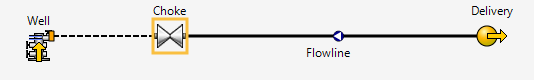
\includegraphics[scale=.9]{Fig/surface_equipment.PNG}
		\caption{Sơ đồ hệ thống thiết bị bề mặt}
		\label{fig:surface_equipment}
	\end{figure}
\newline
Trong phạm vi đồ án nhóm tác giả chỉ lựa chọn phân tích điểm nút tại đáy giếng ngay vị trí của lần bắn mở vỉa thứ nhất.
\newpage
	\begin{figure}[h]
		\centering
		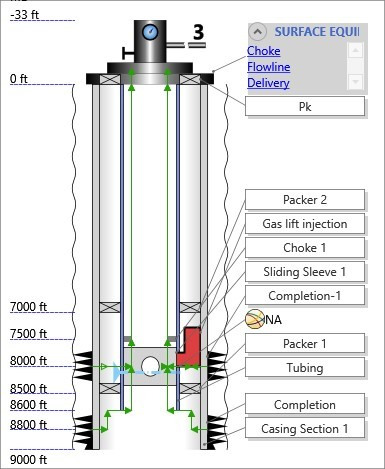
\includegraphics[scale=1.1]{Fig/1d_well_model.png}
		\caption{Mô hình một chiều của giếng}
		\label{fig:1d_well_model}
	\end{figure}
Ngoài ra nhóm tác giả còn đưa ra mô hình hai chiều của giếng theo các thông số khoan định hướng như Hình \ref{fig:2d_well_model}.
\newpage
	\begin{figure}[h]
		\centering
		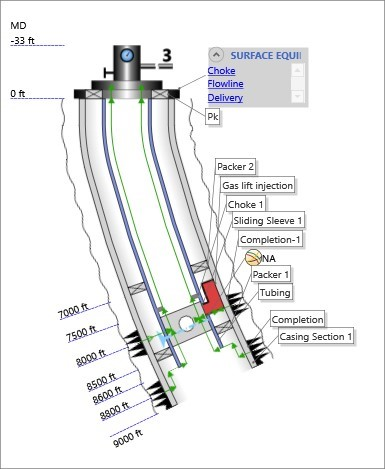
\includegraphics[scale=1.1]{Fig/2d_well_model.png}
		\caption{Mô hình hai chiều của giếng}
		\label{fig:2d_well_model}
	\end{figure}
Chiều sâu thực tế và độ dời đáy của giếng được thể hiện như trong đồ thị Hình \ref{fig:hd_directional_drilling}

\newpage
	\begin{figure}[h]
		\centering
		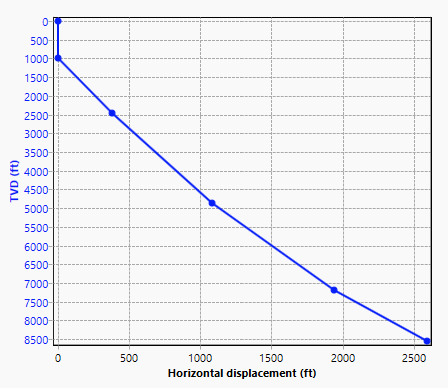
\includegraphics[scale=1.1]{Fig/hd_directional_drilling.PNG}
		\caption{Chiều sâu và độ dời đáy của giếng}
		\label{fig:hd_directional_drilling}
	\end{figure}

\section{Tính toán tối ưu hóa khai thác}
Điều kiện vận hành khai thác của giếng:
	\begin{itemize}
		\item Áp suất vỉa không đổi
		\item Lưu lượng khai thác trên 8000 STB/d
		\item Kích thước van tiết lưu 1 in.
	\end{itemize}
Dựa trên mô hình giếng và các điều kiện thực tế, nhóm tác giả chỉ đi vào phân tích các yếu tố chính là \textit{áp suất vỉa}, \textit{đường kính tubing}, \textit{chỉ số khai thác} và \textit{đường kính van tiết lưu}.

Với giai đoạn đầu khai thác áp suất vỉa còn chưa thay đổi, thay đổi kích thước van tiết lưu ta được các điểm vận hành như sau:
\newpage
	\begin{figure}[h]
		\centering
		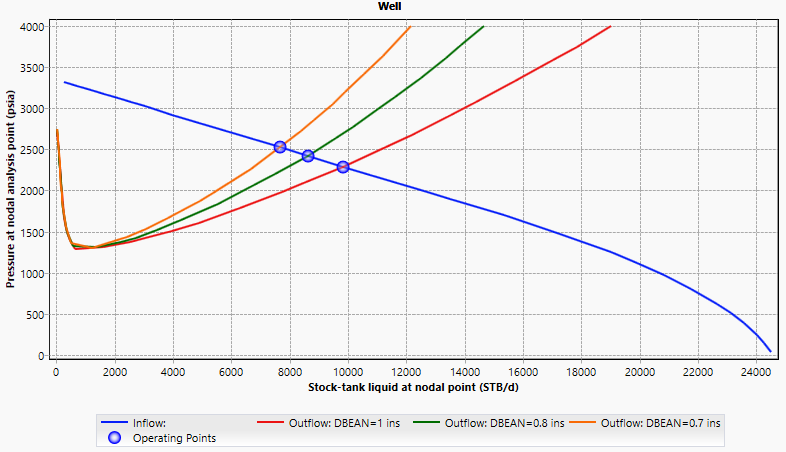
\includegraphics[scale=0.75]{Fig/Static_press_vs_choke.PNG}
		\caption{Điểm vận hành với các kích thước van tiết lưu khác nhau}
		\label{fig:Static_press_vs_choke}
	\end{figure}
Giá trị tại các điểm vận hành được thể hiện trong Bảng \ref{tab:static_press_vs_choke_result}.
\begin{table}[h]
\caption{Kết quả phân tích với áp suất vỉa không đổi}\label{tab:static_press_vs_choke_result}
\begin{tabularx}{\textwidth}{@{}XXX@{}}
\toprule
Điểm vận hành & Lưu lượng (STB/d) & Áp suất (psia) \\ \midrule
DBEAN=1 in    & 9844.934          & 2290.743       \\
DBEAN=0.8 in  & 8624.863          & 2422.37        \\
DBEAN=0.7 in  & 7780.741          & 2524.044       \\ \bottomrule
\end{tabularx}
\end{table}
\newline
Từ kết quả phân tích cho thấy trong giai đoạn áp suất vỉa chưa suy giảm, để đạt được lưu lượng khai thác như mong muốn đường kính van tiết lưu (DBEAN) có thể được đặt ở 0.8 in.
\newpage
Đối với sự thay đổi đường kính trong tubing, kết quả phân tích được thể hiện trong Hình \ref{fig:tubing_vs_static_press} và Bảng \ref{tab:tubing_vs_static_press_result}.
	\begin{figure}[h]
		\centering
		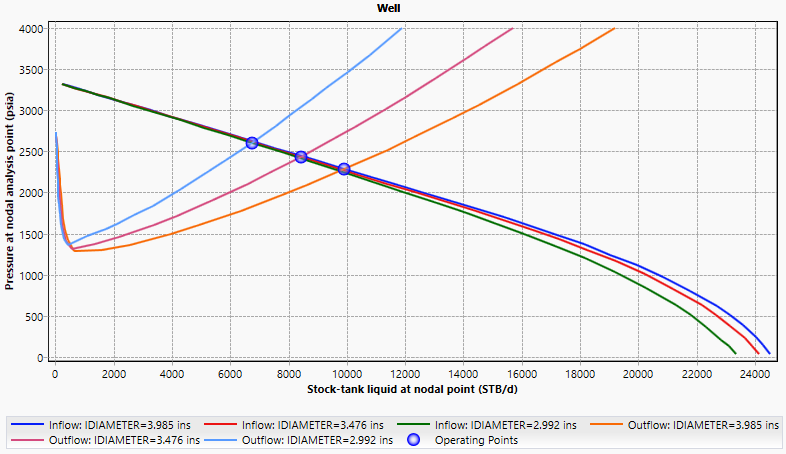
\includegraphics[scale=0.75]{Fig/tubing_vs_static_press.PNG}
		\caption{Điểm vận hành với các đường kính trong tubing khác nhau}
		\label{fig:tubing_vs_static_press}
	\end{figure}

\begin{table}[h]
\caption{Kết quả phân tích với đường kính trong tubing}\label{tab:tubing_vs_static_press_result}
\begin{tabularx}{\textwidth}{@{}XXX@{}}
\toprule
Điểm vận hành & Lưu lượng (STB/d) & Áp suất (psia) \\ \midrule
ID=3.985 in   & 9914.158          & 2283.796       \\
ID=3.476 in   & 8422.956          & 2434.761       \\
ID=2.992 in   & 6736.95           & 2604.85        \\ \bottomrule
\end{tabularx}
\end{table}
Khi thay đổi đường kính trong tubing, đường IPR không thay đổi nhiều. Tuy nhiên, đường OPR có sự thay đổi lớn, để đạt được lưu lượng khai thác lơn hơn 8000 STB/d đường kính trong tubing phù hợp là 3.476 in.
\newpage
Chỉ số khai thác thay đổi kết quả phân tích đạt được thể hiện như trong Hình \ref{fig:pi_vs_choke}.
	\begin{figure}[h]
		\centering
		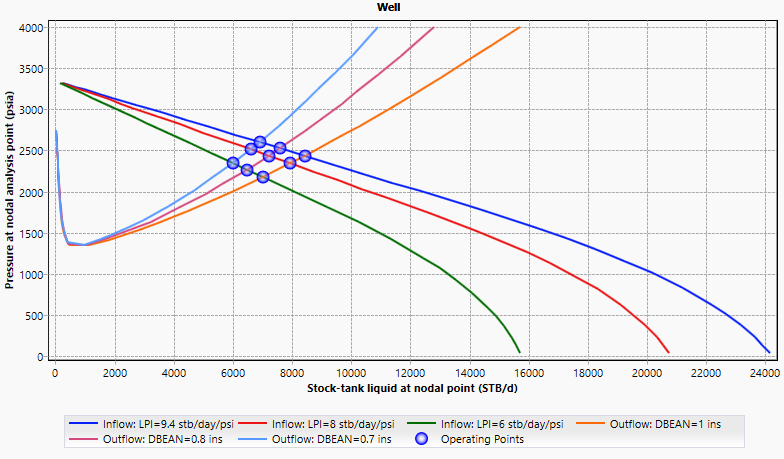
\includegraphics[scale=0.75]{Fig/pi_vs_choke.PNG}
		\caption{Sự thay đổi chỉ số khai thác và đường kính van tiết lưu}
		\label{fig:pi_vs_choke}
	\end{figure}
\begin{table}[h]
\caption{Kết quả phân tích với sự thay đổi của chỉ số khai thác (DBEAN=1 in)}\label{tab:pi_vs_choke_result}
\begin{tabularx}{\textwidth}{@{}XXX@{}}
\toprule
Điểm vận hành          & Lưu lượng (STB/d) & Áp suất (psia) \\ \midrule
PI = 9.4 STB/(d.psi)  & 8423.103          & 2434.744       \\
PI = 8 STB/(d.psi)    & 7938.072          & 2341.531       \\
PI = 6 STB/(d.psi)    & 7006.33           & 2171.567       \\ \bottomrule
\end{tabularx}
\end{table}

Qua Bảng \ref{tab:pi_vs_choke_result} có thể thấy được khi chỉ số khai thác giảm xuống thấp, lưu lượng khai thác bắt đầu giảm. Lúc này, để có thể duy trì lưu lượng khai thác phải tăng đường kính van tiết lưu lớn nhất có thể (1 in) \nomenclature{PI}{Chỉ số khai thác}.

Khi áp suất vỉa bắt đầu suy giảm, vỉa không còn đủ năng lượng để có thể cho lưu lượng khai thác như mong muốn (đối với hệ thống khai thác đang sử dụng). Vì vậy, để duy trì lưu lượng khai thác cần phải thay đổi đường kính tubing. Kết quả phân tích được thể hiện như trong Hình \ref{fig:decrease_press_vs_tubing}.

	\begin{figure}[h]
		\centering
		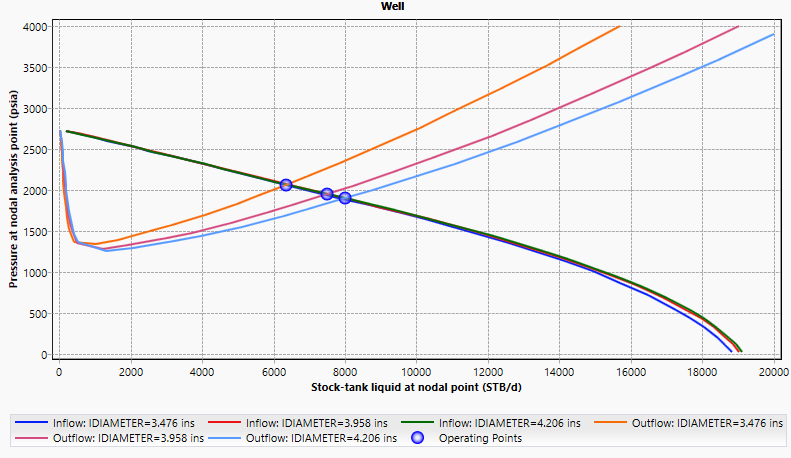
\includegraphics[scale=0.75]{Fig/decrease_press_vs_tubing.PNG}
		\caption{Áp suất suy giảm với các kích thước tubing khác nhau}
		\label{fig:decrease_press_vs_tubing}
	\end{figure}

\begin{table}[h]
\caption{Kết quả phân tích với áp suất vỉa suy giảm}\label{tab:decrease_press_vs_tubing_result}
\begin{tabularx}{\textwidth}{@{}XXX@{}}
\toprule
Điểm vận hành & Lưu lượng (STB/d) & Áp suất (psia) \\ \midrule
ID=3.476 in   & 6353.533          & 2066.458       \\
ID=3.958 in   & 7490.071          & 1951.738       \\
ID=4.206 in   & 8004.196          & 1900.351       \\ \bottomrule
\end{tabularx}
\end{table}

Kết quả thực hiện phân tích như trong Bảng \ref{tab:decrease_press_vs_tubing_result} cho thấy khi áp suất vỉa bắt đầu suy giảm xuống dưới 3000 psi, để có thể duy trì lưu lượng khai thác cần tăng đường kính lên 4.206 in. Lúc này do áp suất vỉa xuống thấp làm cho áp suất qua van tiết lưu suy giảm theo, đồng thời chỉ có thể mở tối đa đường kính van tiết lưu lên 1 in, nên việc thay đổi đường kính van tiết lưu không còn được ưu tiên thực hiện. Kết quả được thể hiện như trong Hình \ref{fig:decrease_press_vs_choke_size}.
\newpage
	\begin{figure}[h]
		\centering
		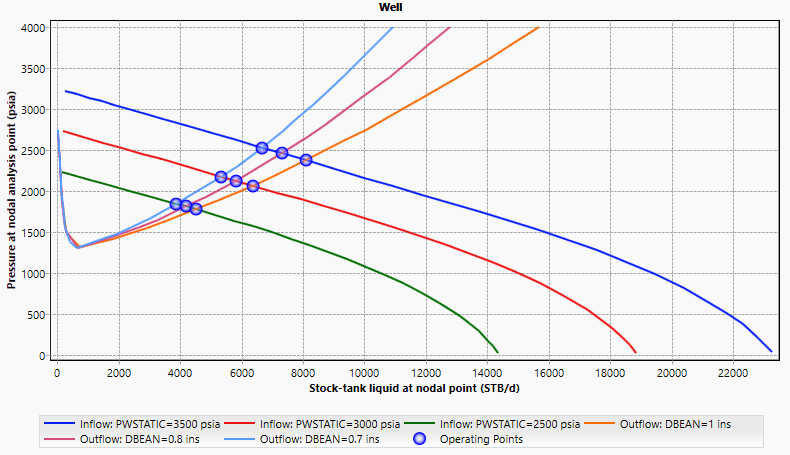
\includegraphics[scale=0.75]{Fig/decrease_press_vs_choke_size.PNG}
		\caption{Thay đổi kích thước van tiết lưu theo sự suy giảm áp suất}
		\label{fig:decrease_press_vs_choke_size}
	\end{figure}

\begin{table}[h]
\caption{Kết quả phân tích suy giảm áp suất với kích thước van tiết lưu (DBEAN = 1 in)}\label{tab:decrease_press_vs_choke_size_result}
\begin{tabularx}{\textwidth}{@{}XXX@{}}
\toprule
Điểm vận hành                  & Lưu lượng (STB/d) & Áp suất (psia) \\ \midrule
PWSTATIC=3500 psia & 8089.64           & 2372.154       \\
PWSTATIC=3000 psia & 6359.535          & 2065.81        \\
PWSTATIC=2500 psia & 4526.497          & 1774.796       \\ \bottomrule
\end{tabularx}
\end{table}
Kết quả phân tích Bảng \ref{tab:decrease_press_vs_choke_size_result} cho thấy khi áp suất bắt đầu suy giảm kích thước van tiết lưu được mở ở mức tối đa cũng không thể duy trì lưu lượng khai thác như mong muốn.
\end{document}